% lint-scope: appendix
\providecommand{\estci}[2]{\begin{tabular}[t]{@{}c@{}}#1\\[-1pt]{\scriptsize #2}\end{tabular}}
The appendices fall into four groups. Appendices~\ref{app:env} to \ref{app:splits} describe the environment, the
scripted rules and how to use Wellocate. Appendices~\ref{app:amendments} to \ref{app:aone} hold the five-model study: what was registered, the runs, PhoQ and the checks behind Section~\ref{sec:res}.
Appendices~\ref{app:grid} to \ref{app:sim} keep the pre-registered prompt study, its follow-up experiments and the learnability simulation. Appendix~\ref{app:b11} covers the trained policy.

\section{Environment details}
\label{app:env}

\paragraph{The landscape.} A candidate's fitness comes from an NK landscape \citep{kauffman1989nk}. $N$ is
the number of positions, here four, and $K$ is how many other positions each position's contribution
depends on. A landscape is rugged when it has local peaks, candidates that no single-letter change can
improve, and a larger $K$ makes it more rugged. We set $K=1$, so each position's contribution depends on the
next position along the string, wrapping round at the end. Each position has its own table of
contributions, one for every pair of letters at that position and the next, drawn uniformly between 0 and 1
when the landscape is generated. A candidate's fitness is the mean of its four contributions. The whole
landscape is then multiplied by one constant so its maximum is 8.762, the highest value measured in the
published data. This only sets the units, and beyond that value and its share of working candidates the
landscape is a standard NK landscape. At $K=1$ position interactions are weak, so the search itself is simple, and an
agent that falls short does so through how it spends measurements. The agents were run at $K=1$ only, and
the learnability simulation in Appendix~\ref{app:sim} repeats the scripted analysis at $K=2$ and 3.

\paragraph{Viability.} A candidate is viable if its fitness exceeds the 93rd percentile, which leaves
11{,}199 viable candidates, 7.00\% of the space. The threshold was chosen so that about the same share of
candidates works as in the published data. In GB1, \nGbViable\% of variants keep at least a tenth of the wild type's
fitness. GB1 and PhoQ are cut at the same share, so their never-measured variants, stored as zero, are all
non-viable. On PhoQ the authors' own call of functional variants is much narrower, so there the cut also admits
variants they would call non-functional. Treating ``does not work'' as a sharp cutoff on fitness is a
simplification.

\paragraph{Ordering and failures.} Each slot is filled by an order, a request to measure one candidate
once. An order for a non-viable candidate is rejected. The agent is told, and is asked for a replacement in
the same round, up to three times. If every replacement is also non-viable, the slot is lost and still
counts against the budget. About 15\% of orders fail at random, whatever the candidate's fitness, and a
failed order returns nothing and still uses its slot. The rate is a design choice. Over the 5{,}075 agent
campaigns of the prompt study (Appendix~\ref{app:grid}), 14.97\% of 300{,}898 measurements attempted on viable candidates failed.

\paragraph{Noise.}
\label{app:noise}
Each measurement of a viable candidate returns its true fitness plus independent Gaussian error, whose
standard deviation grows with the true fitness $f$:
\[ \sigma(f) = \sqrt{0.00351^2 + (0.073 f)^2}. \]
Both constants in $\sigma(f)$ are sized from the read counts of \citet{wu2016adaptation}, who screened a library
spanning all 160{,}000 variants in one deep mutational scan and got a usable reading for 93.4\% of them. In such an experiment every variant is mixed into one
pool, and the pool goes through a selection step that keeps variants binding a target. A variant that binds
better is kept in larger numbers. Each protein stays physically linked to the DNA that encodes it, so
counting that DNA counts the protein. The DNA is counted before and after selection by sequencing, which
reads DNA in short pieces. Each piece is one read, a variant's count is how many reads matched it, and the
reads per variant is the \emph{read depth}.

In that study a variant's fitness is its after-to-before read ratio, divided by the same ratio for the
unmodified protein the study started from. That protein is unrelated to \texttt{GDIF}. The study's
published read totals average 557 reads per variant before selection and 285 after. Treating each count as Poisson, the variance
of the log ratio is about $1/285 + 1/557$, so its standard deviation, the relative error, is about 7.3\%. We apply this
average depth to every candidate, which gives the constant 0.073. Real counts are often more spread out than Poisson, so this is a
lower estimate of that study's counting error.

Taking the starting protein's ratio as the study's average, $285/557$, a variant with 557 reads before
selection and a single read after has fitness $(1/557)/(285/557)$, or 0.0035 units. That is the smallest
non-zero value the study could resolve, and we use it as the smallest spread any reading has. It matters
only near zero fitness, so it has no practical effect on a viable candidate.

A variant that binds better gets more reads, so one average depth overstates the counting error of the best
candidates. A real re-run also varies for reasons beyond counting. The simulation may therefore be noisier or less
noisy than a real lab, and which of the two holds is not known.

\paragraph{The reference candidate.} \texttt{GDIF} is the viable candidate at the median fitness. Its true
fitness, 6.8730, is stated to the agent to two decimals, and Table~\ref{tab:cells} gives the re-testing
share with and without re-orders of it. We also checked that the scripted results do not depend on this
start. On each landscape we drew \nStartsRandom{} viable starts at random and ran the three scripted rules from each,
on our campaign seeds. The guessing and informed rules keep \texttt{GDIF}'s best number of re-tests from
every start on all three landscapes, and on the grid the guessing rule's re-testing share at that setting stays
between \nStartGuessShareMinGrid\% and \nStartGuessShareMaxGrid\%. On the grid the model-guided rule's best setting moves
between no re-test and one a round, which score almost the same: at our setting of one re-test its share stays
between \nStartMgShareMinGrid\% and \nStartMgShareMaxGrid\%, and keeping that setting costs a median of
\nStartMgPickLostMedGrid{} in final pick, at most \nStartMgPickLostMaxGrid. On GB1 and PhoQ it keeps \texttt{GDIF}'s setting from \nStartSameKGbMg{} and \nStartSameKPqMg{} of the \nStartsRandom{} starts.

\paragraph{What the simulation leaves out.} A non-viable order is caught and replaced. In a lab, finding out would
cost a well. A new variant and a re-test cost the same slot. A lab must first make a new variant, which makes exploring dearer there and could raise a lab's best rate of re-testing. A lab
usually wants a shortlist, and ranking a shortlist could reward more re-testing than one final pick does.
Real rounds use plates of 96 or 384 wells, so the best number of repeats found here does not transfer as a
number. Whether the agents' misallocation depends on batch size or budget is not tested. Noise here has no plate effects
or drift, meaning slow shifts in readings between plates or over time, and in a real lab a repeat can also
catch those. So an agent that re-tests more than the scripted rules here would not necessarily re-test too much in a
real lab.

\section{The scripted rules}
\label{app:refs}

The guessing and informed rules of Section~\ref{sec:env} were the prompt study's references, and the model-guided
rule was added later under a registered change. The guessing and informed rules spend $k$ of the four slots a round
re-testing their current best, and $k^\ast$ is the best setting. The informed rule is told which candidates are
viable. It is never rejected, so it loses no slots to rejections, and it still has to find out how good each candidate is. The agents are not told
which candidates are viable, so the informed rule has an easier task than theirs. The guessing rule was pre-registered and run before any result was
written. It tries every candidate one letter away from its current best, and follows the agents' rules for rejections,
replacements and lost slots, in the same code. Both ran on the same 1{,}500 seeds per setting.

The model-guided rule spends its first four rounds trying one-letter changes of the start, one at each position. From
the fifth round it orders three new candidates a round, ranked by its letter scores, and re-tests one leading
candidate: its best, or the next best once the best has two readings. In its last three rounds it re-tests its four
best candidates by mean reading. It picks with the registered selection rule of Section~\ref{sec:under}.

\begin{table}[h]
\centering
\small
\caption{The guessing and informed rules on the grid. One knows more than the agents, the other knows the same.}
\begin{tabular}{lrr}
\toprule
 & informed (told which are viable) & guessing (must guess) \\
\midrule
best re-tests a round, $k^\ast$     & 1 of 4 slots & 1 of 4 slots \\
mean pick at $k{=}0$                & 7.8862 & 7.7098 \\
mean pick at $k^\ast$               & 7.9993 & 7.8659 \\
distinct candidates at $k^\ast$     & 39.14  & 28.94 \\
rejections per campaign at $k{=}1$  & 0.00   & 83.02 \\
lost slots per campaign at $k{=}1$  & 0.00   & 11.70 \\
campaigns collapsing at $k{=}4$     & 16 of 1{,}500 & 147 of 1{,}500 \\
\bottomrule
\end{tabular}
\end{table}

On the grid both do best at one re-test a round, and every grid comparison with the agents holds against either.



\section{Using Wellocate}
\label{app:using}
\label{app:splits}

\paragraph{Interface.} An episode is one campaign. A call to \texttt{step} orders up to four candidates, or one
replacement after a rejection, and \texttt{nominate} ends the episode. Observations hold readings, outcomes and the
remaining budget, and no true value; the reward is the nominee's true value. A text mode returns the exact prompts our agents received and reads replies the same way, asking again when a reply cannot be read. A language model and a policy trained by reinforcement learning thus face the same task. The environment runs the same code as our experiments. Through it the
guessing rule reproduces our reference pick of 7.8659 and re-testing share of 23.78\% exactly, the informed rule its
pick of 7.9993, and one core
runs about \nEpisodesPerSec{} episodes a second.

\paragraph{Tracks and splits.} The protein track uses scrambled GB1 and PhoQ, with fresh scrambles for training,
validation and testing and the real amino-acid names held out (Table~\ref{tab:splits}). A scramble changes only the names, so a protein test split asks for unseen names of the same protein. Training on one protein and testing on the other asks for transfer. The grid track gives fresh NK landscapes and holds out rougher ones. Every split is fixed and public. A hidden test server is future work.

\paragraph{Scoring and baselines.} The scorecard gives each policy's mean pick and its regret against the informed rule on the same episodes. It adds the re-testing share, the exploration and selection losses, the candidates measured and the slots lost, each with a 95\% interval. Beside them it names the best scripted share for that landscape and noise.
The baselines are random ordering, the guessing rule, the informed rule and the model-guided rule. A fifth, a simple untuned confirmation policy, explores without repeats and re-tests its top candidates at the end. Our language-model results
sit beside them as read-only rows.

\paragraph{Noise and the best split.} On the grid the guessing rule that never re-tests loses \nGridSelLow{},
\nGridSelAssay{} and \nGridSelHigh{} at selection at low, assay and high noise. On PhoQ one re-test a round ties with
no re-tests at about \nPhoqTimesLow{} times assay noise, and wins clearly at \nPhoqTimesHigh{} times. On GB1 it wins
only at \nGbTimesHigh{} times (Table~\ref{tab:onevszero}). Part of re-testing's value on the grid is avoiding
rejections: the rule that never re-tests loses \nGridLostKzero{} slots to rejections, against \nGridLostKone{} for one
re-test a round. With free rejections, one re-test a round still beats no re-tests on the grid at assay noise
(Table~\ref{tab:onevszero}), so there re-testing also pays because of the noise. With free rejections the best number
of re-tests also rises with noise sooner on the grid, and GB1 and PhoQ keep the best settings of
Figure~\ref{fig:noise} (Figure~\ref{fig:noisefree}).

\begin{table}[tbp]
\centering
\small
\caption{The guessing rule's final pick with no re-tests and with one re-test a round, with 95\% intervals.}
\label{tab:onevszero}
\begin{tabular}{lcc}
\toprule
 & no re-tests & one re-test a round \\
\midrule
GB1, \nGbTimesHigh{} times assay noise & \estci{\nGbHighKzero}{\nGbHighKzeroci} & \estci{\nGbHighKone}{\nGbHighKoneci} \\
grid, free rejections, assay noise & \estci{\nGridRfKzero}{\nGridRfKzeroci} & \estci{\nGridRfKone}{\nGridRfKoneci} \\
\bottomrule
\end{tabular}
\end{table}

\begin{figure}[htbp]
\centering
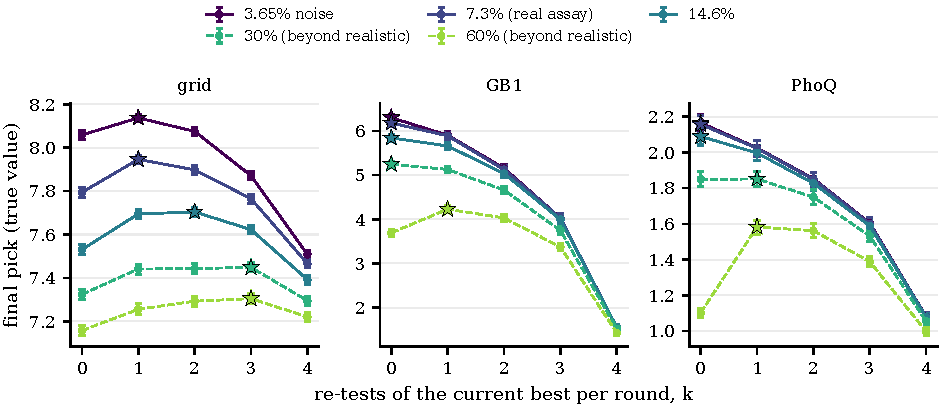
\includegraphics[width=\textwidth]{fig_noise_sweep_free.pdf}
\caption{Figure~\ref{fig:noise} with free rejections: a rejected order never costs a slot.}
\label{fig:noisefree}
\end{figure}

% Generated by scripts/make_table_splits.py from wellocate/splits.json. Do not edit by hand;
% scripts/verify_paper_numbers.py regenerates it and fails on any difference.
\begin{table}[!htbp]
\centering
\small
\setlength{\tabcolsep}{5pt}
\caption{Wellocate's frozen splits: landscapes / episodes per split. Train, validation and test use disjoint landscape seeds (scrambles for GB1 and PhoQ, NK seeds for the grid) and disjoint campaign seeds. Held out: the real amino-acid names for GB1 and PhoQ, and two rougher NK settings, $K = 2$ and $K = 3$. \emph{Paper} is the landscape and seeds used in this study.}
\label{tab:splits}
\begin{tabular}{llrrrrr}
\toprule
track & landscape & train & validation & test & held out & paper \\
\midrule
protein & scrambled GB1 & 400 / 100{,}000 & 10 / 1{,}500 & 20 / 1{,}500 & 1 / 1{,}500 & 1 / 1{,}500 \\
protein & scrambled PhoQ & 400 / 100{,}000 & 10 / 1{,}500 & 20 / 1{,}500 & 1 / 1{,}500 & 1 / 1{,}500 \\
grid & generated NK & 400 / 100{,}000 & 10 / 1{,}500 & 20 / 1{,}500 & \begin{tabular}[t]{@{}r@{}}$K = 2$: 20 / 1{,}500 \\ $K = 3$: 20 / 1{,}500\end{tabular} & 1 / 1{,}500 \\
\bottomrule
\end{tabular}
\end{table}

